% sections/decision_engine.tex

\section{Decision Engine}
\label{sec:decision_engine}

The decision engine evaluates a set of routing decisions against the signal result and selects the best match.
In Shannon's 1938 master's thesis~\cite{shannon1938symbolic}, arbitrary switching-circuit behavior was shown to be representable and minimizable through Boolean algebra---any desired input--output relation over binary signals could be systematically synthesized from $\{\wedge, \vee, \neg\}$.
The decision engine applies this same principle to routing: each routing policy is expressed as a Boolean formula over binary signal conditions, and the functionally complete operator set guarantees that \emph{any} routing policy expressible as a function of the extracted signals can be realized---without modifying the signal layer or the execution layer.
We formalize the decision model, present the evaluation algorithm, and analyze the selection strategies.

\subsection{Decision Model}

\begin{definition}[Decision]
A \emph{decision} $d = (n, \phi, \mathcal{M}_d, \Pi_d, p)$ consists of a name $n$, a Boolean formula $\phi$ over signal conditions, a candidate model set $\mathcal{M}_d \subseteq \mathcal{M}$, a plugin configuration $\Pi_d$, and a priority $p \in \mathbb{Z}$.
\end{definition}

\begin{definition}[Rule Node --- Boolean Expression Tree]
A \emph{rule node} $\phi$ is defined recursively as one of two forms (\Cref{fig:rule_node_tree} illustrates example expression trees):
\begin{itemize}[nosep,leftmargin=1.5em]
  \item \textbf{Leaf} (signal reference): $\phi = \textsc{leaf}(\tau, n)$, referencing a signal type $\tau$ and rule name $n$.
  \item \textbf{Composite} (Boolean operator): $\phi = (\textsc{op}, [\phi_1, \ldots, \phi_k])$, where $\textsc{op} \in \{\textsc{and}, \textsc{or}, \textsc{not}\}$ and $\phi_1, \ldots, \phi_k$ are child rule nodes. $\textsc{not}$ is strictly unary ($k = 1$).
\end{itemize}
Evaluation proceeds by structural recursion:
\begin{equation}
  \text{eval}(\phi, S(r)) =
  \begin{cases}
    \mathbf{1}\bigl[\exists\, (\rho, 1, c) \in S(r) : \rho.\tau = \tau \wedge \rho.n = n\bigr]
      & \text{if } \phi = \textsc{leaf}(\tau, n) \\[4pt]
    \bigwedge_{i=1}^{k} \text{eval}(\phi_i, S(r))
      & \text{if } \textsc{op} = \textsc{and} \\[4pt]
    \bigvee_{i=1}^{k} \text{eval}(\phi_i, S(r))
      & \text{if } \textsc{op} = \textsc{or} \\[4pt]
    \neg\, \text{eval}(\phi_1, S(r))
      & \text{if } \textsc{op} = \textsc{not}
  \end{cases}
\end{equation}
\end{definition}

The recursive structure enables arbitrarily nested Boolean expressions.
Classical flat formulas---a single AND or OR over leaf conditions---are the depth-1 special case and remain the recommended form for simple routing policies.
When richer logic is needed, nesting expresses compound operators directly within a single decision:
$\textsc{nor}(A,B) = \textsc{not}(\textsc{or}(A,B))$;
$\textsc{nand}(A,B) = \textsc{not}(\textsc{and}(A,B))$;
$\textsc{xor}(A,B) = \textsc{or}(\textsc{and}(A, \textsc{not}(B)),\; \textsc{and}(\textsc{not}(A), B))$.
YAML's natural indentation mirrors the logical nesting, preserving readability and auditability even for complex formulas.
Priority-ordered decisions compose multiple such formulas into an ordered evaluation, providing conflict resolution and organizational structure for deployment-scale routing policies.

\begin{figure}[ht]
  \centering
  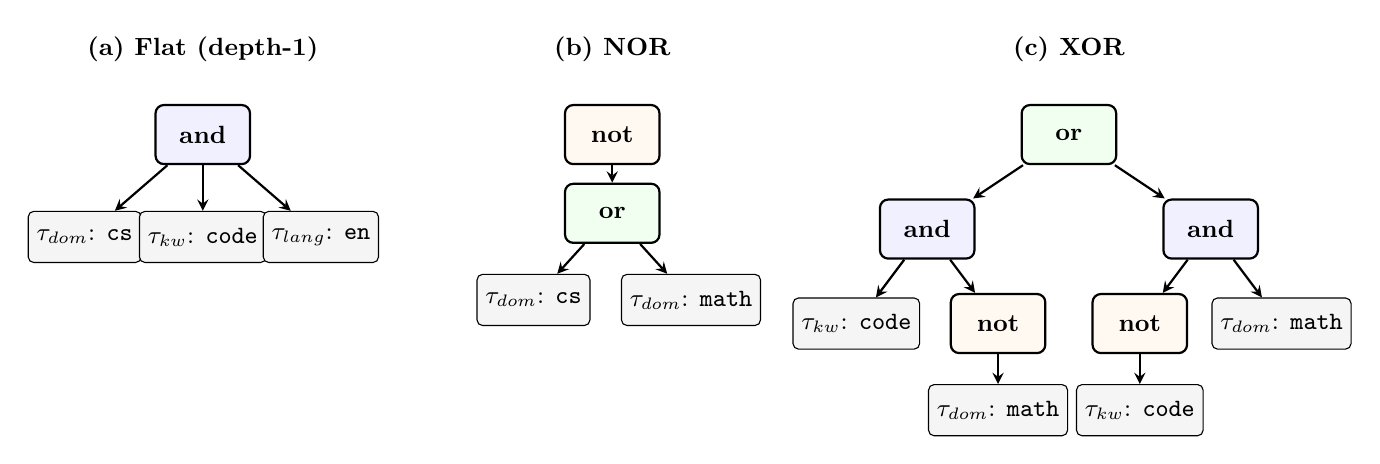
\begin{tikzpicture}[
    gate/.style={rectangle, draw, thick, rounded corners=3pt,
                 minimum height=0.75cm, minimum width=1.2cm,
                 align=center, inner sep=3pt, font=\small\bfseries},
    leaf/.style={rectangle, draw, rounded corners=2pt, fill=black!4,
                 minimum height=0.65cm, align=center,
                 inner sep=3pt, font=\small},
    arr/.style={->, >=stealth, thick},
    lbl/.style={font=\scriptsize, text=gray!70},
  ]

  % --- (a) Flat depth-1: AND(A, B, C) ---
  \node[font=\small\bfseries, anchor=south] at (0, 2.6) {(a) Flat (depth-1)};
  \node[gate, fill=blue!6] (and1) at (0, 1.8) {\textsc{and}};
  \node[leaf] (a1) at (-1.5, 0.5) {$\tau_\text{dom}$: \texttt{cs}};
  \node[leaf] (b1) at (0, 0.5) {$\tau_\text{kw}$: \texttt{code}};
  \node[leaf] (c1) at (1.5, 0.5) {$\tau_\text{lang}$: \texttt{en}};
  \draw[arr] (and1) -- (a1);
  \draw[arr] (and1) -- (b1);
  \draw[arr] (and1) -- (c1);

  % --- (b) NOR: NOT(OR(A, B)) ---
  \node[font=\small\bfseries, anchor=south] at (5.2, 2.6) {(b) NOR};
  \node[gate, fill=orange!5] (not2) at (5.2, 1.8) {\textsc{not}};
  \node[gate, fill=green!6] (or2) at (5.2, 0.8) {\textsc{or}};
  \node[leaf] (a2) at (4.2, -0.3) {$\tau_\text{dom}$: \texttt{cs}};
  \node[leaf] (b2) at (6.2, -0.3) {$\tau_\text{dom}$: \texttt{math}};
  \draw[arr] (not2) -- (or2);
  \draw[arr] (or2) -- (a2);
  \draw[arr] (or2) -- (b2);

  % --- (c) XOR: OR(AND(A, NOT(B)), AND(NOT(A), B)) ---
  \node[font=\small\bfseries, anchor=south] at (11.0, 2.6) {(c) XOR};
  \node[gate, fill=green!6] (or3) at (11.0, 1.8) {\textsc{or}};
  \node[gate, fill=blue!6] (and3l) at (9.2, 0.6) {\textsc{and}};
  \node[gate, fill=blue!6] (and3r) at (12.8, 0.6) {\textsc{and}};
  \draw[arr] (or3) -- (and3l);
  \draw[arr] (or3) -- (and3r);

  % Left branch: AND(A, NOT(B))
  \node[leaf] (a3) at (8.3, -0.6) {$\tau_\text{kw}$: \texttt{code}};
  \node[gate, fill=orange!5] (not3l) at (10.1, -0.6) {\textsc{not}};
  \node[leaf] (b3l) at (10.1, -1.7) {$\tau_\text{dom}$: \texttt{math}};
  \draw[arr] (and3l) -- (a3);
  \draw[arr] (and3l) -- (not3l);
  \draw[arr] (not3l) -- (b3l);

  % Right branch: AND(NOT(A), B)
  \node[gate, fill=orange!5] (not3r) at (11.9, -0.6) {\textsc{not}};
  \node[leaf] (a3r) at (11.9, -1.7) {$\tau_\text{kw}$: \texttt{code}};
  \node[leaf] (b3r) at (13.7, -0.6) {$\tau_\text{dom}$: \texttt{math}};
  \draw[arr] (and3r) -- (not3r);
  \draw[arr] (and3r) -- (b3r);
  \draw[arr] (not3r) -- (a3r);

  \end{tikzpicture}
  \caption{Rule-node expression trees at increasing depth. (a)~A flat depth-1 tree: AND over three leaf conditions. (b)~A NOR expression: $\textsc{not}(\textsc{or}(\text{cs},\text{math}))$, matching all non-STEM queries. (c)~An XOR expression composed from AND, OR, and NOT primitives, routing requests that match exactly one of two signals. Leaf nodes (gray) reference signal conditions; composite nodes use AND (\textcolor{blue!50}{blue}), OR (\textcolor{green!50}{green}), and NOT (\textcolor{orange!45}{orange}).}
  \label{fig:rule_node_tree}
\end{figure}

\subsection{Confidence Computation}

When a decision matches, we compute a confidence score as the mean confidence over satisfied conditions:

\begin{equation}
  \text{conf}(d, S(r)) = \frac{1}{|\Gamma_\text{sat}|} \sum_{\gamma_j \in \Gamma_\text{sat}} c_j(r)
  \label{eq:confidence}
\end{equation}

where $\Gamma_\text{sat} = \{\gamma_j \in \Gamma \mid \text{sat}(\gamma_j, S(r)) = 1\}$ and $c_j(r)$ is the signal confidence for condition $\gamma_j$.
For embedding signals, $c_j$ is the cosine similarity; for heuristic and binary ML signals, $c_j = 1.0$.

\subsection{Selection Strategies}

Given the set of matched decisions $\mathcal{D}_\text{match} = \{d \in \mathcal{D} \mid \text{eval}(\phi_d, S(r)) = 1\}$, two strategies select $d^*$:

\noindent\textbf{Priority Strategy.}
\begin{equation}
  d^* = \arg\max_{d \in \mathcal{D}_\text{match}} p_d
\end{equation}
This provides deterministic, administrator-controlled routing.
Ties are broken by insertion order.

\noindent\textbf{Confidence Strategy.}
\begin{equation}
  d^* = \arg\max_{d \in \mathcal{D}_\text{match}} \text{conf}(d, S(r))
\end{equation}
This enables data-driven routing where embedding similarity and classifier confidence drive selection.

The priority strategy is the default for production deployments where predictability is paramount.
The confidence strategy is preferred for experimental settings where the system should adapt to query characteristics.

\subsection{Evaluation Algorithm}

\begin{algorithm}[t]
\caption{Decision Evaluation}
\label{alg:decision_eval}
\begin{algorithmic}[1]
\REQUIRE Signal result $S(r)$, decisions $\mathcal{D}$, strategy $\sigma \in \{\text{priority}, \text{confidence}\}$
\ENSURE Selected decision $d^*$, confidence $c^*$
\STATE $\mathcal{D}_\text{match} \leftarrow \emptyset$
\FOR{$d \in \mathcal{D}$}
  \IF{$\text{eval}(\phi_d, S(r))$}
    \STATE $c_d \leftarrow \text{conf}(d, S(r))$
    \STATE $\mathcal{D}_\text{match} \leftarrow \mathcal{D}_\text{match} \cup \{(d, c_d)\}$
  \ENDIF
\ENDFOR
\IF{$\sigma = \text{priority}$}
  \STATE $(d^*, c^*) \leftarrow \arg\max_{(d, c) \in \mathcal{D}_\text{match}} p_d$
\ELSE
  \STATE $(d^*, c^*) \leftarrow \arg\max_{(d, c) \in \mathcal{D}_\text{match}} c$
\ENDIF
\RETURN $(d^*, c^*)$
\end{algorithmic}
\end{algorithm}

The algorithm runs in $O(M \cdot L_{\max})$ where $M = |\mathcal{D}|$ is the number of decisions and $L_{\max}$ is the maximum number of conditions per decision.
In practice, $M \leq 50$ and $L_{\max} \leq 10$, making decision evaluation negligible ($< 0.1$\,ms) relative to signal extraction.

\subsection{Expressiveness Analysis}

The recursive rule-node model can express common routing patterns with depth-1 trees (flat formulas) and richer patterns through nesting:

\begin{itemize}[leftmargin=*]
  \item \textbf{Domain routing}: A single leaf condition routes by classified domain.
  \item \textbf{Guarded routing}: AND of a domain condition and a complexity condition routes complex queries within a domain to a capable model.
  \item \textbf{Exclusion routing}: $\textsc{and}(\text{domain}, \textsc{not}(\text{complexity}))$ routes simple queries within a domain to a lightweight model, avoiding the cost of a full-capability model for straightforward requests.
  \item \textbf{Multi-signal routing}: AND of keyword, embedding, and language conditions provides precise routing for specific query patterns.
  \item \textbf{Fallback chains}: Multiple decisions with decreasing priority and progressively broader conditions implement fallback routing.
  \item \textbf{NOR routing} (blanket exclusion): $\textsc{not}(\textsc{or}(\text{cs}, \text{math}, \text{physics}))$ routes all non-STEM queries to a general-purpose model without enumerating every non-STEM domain.
  \item \textbf{NAND routing} (conditional exemption): $\textsc{not}(\textsc{and}(\text{zh}, \text{code}))$ matches all requests \emph{except} Chinese-language code queries, useful for compliance-based routing.
  \item \textbf{XOR routing} (mutual exclusion): $\textsc{or}(\textsc{and}(A, \textsc{not}(B)),\; \textsc{and}(\textsc{not}(A), B))$ routes requests matching exactly one of two signals, enabling exclusive specialization.
  \item \textbf{Nested multi-signal}: $\textsc{and}(\textsc{or}(\text{cs}, \text{math\_kw}),\; \text{en},\; \textsc{not}(\text{long\_ctx}))$ combines disjunctive, conjunctive, and negated sub-trees in a single decision for fine-grained routing.
\end{itemize}

\noindent\textbf{Functional completeness.}
The expressiveness of the recursive rule-node model rests on a classical result from Boolean algebra~\cite{huntington1904sets}: the operator set $\{\wedge, \vee, \neg\}$ is \emph{functionally complete}---any Boolean function $f: \{0,1\}^N \to \{0,1\}$ can be expressed as a formula over these operators.
Because each rule node may nest AND, OR, and NOT to arbitrary depth, a \emph{single} decision formula $\phi$ can already represent any Boolean function over the $N$ signal match indicators---no multi-decision composition is required for completeness.

\begin{proposition}[Single-decision completeness]
For any Boolean function $f: \{0,1\}^N \to \{0,1\}$ over signal match indicators, there exists a rule node $\phi$ using AND, OR, and NOT such that $\text{eval}(\phi, S(r)) = f(S(r))$ for all signal results $S(r)$.
\end{proposition}

\begin{proof}[Proof sketch]
Construct $\phi$ directly from the truth table of $f$.
For each minterm (input assignment where $f = 1$), form an AND-node over the corresponding literals (a leaf $\textsc{leaf}(\tau_i, n_i)$ when the $i$-th signal is 1, or $\textsc{not}(\textsc{leaf}(\tau_i, n_i))$ when it is 0).
Collect all such AND-nodes under a single OR-node.
Since $\{\wedge, \vee, \neg\}$ is functionally complete, the resulting tree evaluates to $f$.
\end{proof}

\begin{proposition}[Routing policy completeness]
For any routing policy $\pi: \{0,1\}^N \to \mathcal{M} \cup \{\bot\}$ mapping signal vectors to model selections, there exists a decision set $\mathcal{D}$ with recursive AND/OR/NOT formulas and priority ordering such that $\pi$ is realized by the evaluation algorithm (\Cref{alg:decision_eval}).
\end{proposition}

\begin{proof}[Proof sketch]
For each model $m_k$ in the range of $\pi$, construct a single decision $d_k$ whose rule node encodes the Boolean function $f_k(\mathbf{s}) = \mathbf{1}[\pi(\mathbf{s}) = m_k]$ using the single-decision completeness result above.
Assign priorities to resolve overlaps deterministically.
\end{proof}

This two-level universality guarantee---completeness within a single decision \emph{and} across a decision set---means the decision engine imposes \emph{no inherent limitation} on what routing policies can be configured.
Priority ordering across decisions is no longer required for expressiveness; it serves as an organizational and conflict-resolution mechanism, equivalent to a decision list~\cite{rivest1987learning} over Boolean features.

\noindent\textbf{Structural analogy to combinational logic circuits.}
The recursive rule-node model maps naturally onto the hierarchy of combinational logic circuits studied in digital design~\cite{brayton1984logic}.
The following table summarizes the correspondence at three levels of generality:

\begin{center}
\begin{tabular}{llp{4.2cm}}
\toprule
\textbf{Circuit Model} & \textbf{Routing System} & \textbf{Expressiveness} \\
\midrule
PLA (two-level)~\cite{fleisher1975introduction}
  & Flat decision (depth-1 tree)
  & Any two-level Boolean function \\
General combinational circuit
  & Recursive rule-node tree
  & Any Boolean function \\
Circuit array + priority encoder
  & Decision set + priority ordering
  & Any routing policy $\pi: \{0,1\}^N \!\to\! \mathcal{M}$ \\
\bottomrule
\end{tabular}
\end{center}

At the first level, a depth-1 rule node---a single AND or OR over leaf conditions---is structurally isomorphic to a \emph{Programmable Logic Array} (PLA)~\cite{fleisher1975introduction}: signal extractors correspond to input lines, leaf conditions to the AND-plane, and the top-level operator to the OR-plane.
At the second level, a recursive rule-node tree corresponds to a general combinational logic circuit---a directed acyclic graph of AND, OR, and NOT gates---where each decision is a complete circuit computing an arbitrary Boolean function.
At the third level, the priority-ordered decision set acts as an array of such circuits with a priority encoder selecting the output, realizing any routing policy.
\Cref{fig:circuit_analogy} illustrates this three-level correspondence.

\begin{figure*}[ht]
  \centering
  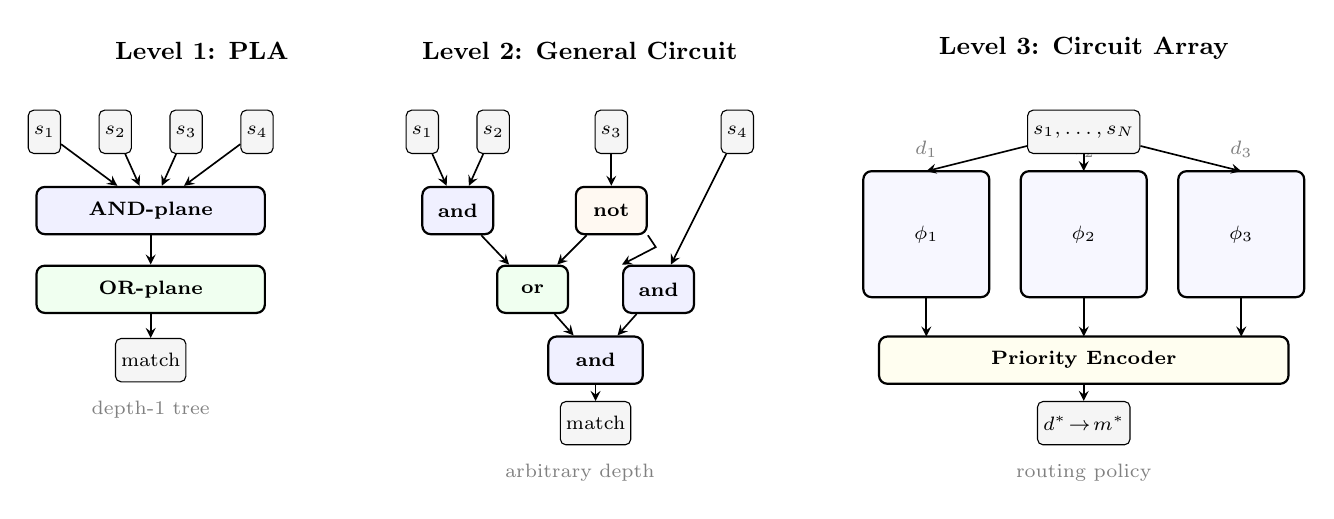
\begin{tikzpicture}[
    gate/.style={rectangle, draw, thick, rounded corners=3pt,
                 minimum height=0.6cm, minimum width=0.9cm,
                 align=center, inner sep=2pt, font=\scriptsize\bfseries},
    io/.style={rectangle, draw, rounded corners=2pt, fill=black!4,
               minimum height=0.55cm, align=center,
               inner sep=2pt, font=\scriptsize},
    prio/.style={rectangle, draw, thick, rounded corners=3pt, fill=yellow!6,
                 minimum height=0.6cm, align=center,
                 inner sep=3pt, font=\scriptsize\bfseries},
    arr/.style={->, >=stealth, semithick},
    darr/.style={->, >=stealth, densely dashed, gray!50},
    brace/.style={decorate, decoration={brace, amplitude=5pt, mirror}},
    titl/.style={font=\small\bfseries, anchor=south},
  ]

  % ===== Level 1: PLA (flat) =====
  \node[titl] at (1.8, 3.6) {Level 1: PLA};

  % Input signals
  \node[io] (s1a) at (-0.2, 2.8) {$s_1$};
  \node[io] (s2a) at (0.7, 2.8) {$s_2$};
  \node[io] (s3a) at (1.6, 2.8) {$s_3$};
  \node[io] (s4a) at (2.5, 2.8) {$s_4$};

  % AND-plane
  \node[gate, fill=blue!6, minimum width=2.9cm] (andp) at (1.15, 1.8) {AND-plane};
  % OR-plane
  \node[gate, fill=green!6, minimum width=2.9cm] (orp) at (1.15, 0.8) {OR-plane};
  % Output
  \node[io] (out1) at (1.15, -0.1) {match};

  \draw[arr] (s1a) -- (andp);
  \draw[arr] (s2a) -- (andp);
  \draw[arr] (s3a) -- (andp);
  \draw[arr] (s4a) -- (andp);
  \draw[arr] (andp) -- (orp);
  \draw[arr] (orp) -- (out1);

  \node[font=\scriptsize, text=gray, anchor=north] at (1.15, -0.5) {depth-1 tree};

  % ===== Level 2: General circuit (recursive) =====
  \node[titl] at (6.6, 3.6) {Level 2: General Circuit};

  % Input signals
  \node[io] (s1b) at (4.6, 2.8) {$s_1$};
  \node[io] (s2b) at (5.5, 2.8) {$s_2$};
  \node[io] (s3b) at (7.0, 2.8) {$s_3$};
  \node[io] (s4b) at (8.6, 2.8) {$s_4$};

  % Gate network
  \node[gate, fill=blue!6] (g1) at (5.05, 1.8) {\textsc{and}};
  \node[gate, fill=orange!5] (g2) at (7.0, 1.8) {\textsc{not}};
  \node[gate, fill=green!6] (g3) at (6.0, 0.8) {\textsc{or}};
  \node[gate, fill=blue!6] (g4) at (7.6, 0.8) {\textsc{and}};
  \node[gate, fill=blue!6, minimum width=1.2cm] (g5) at (6.8, -0.1) {\textsc{and}};

  \draw[arr] (s1b) -- (g1);
  \draw[arr] (s2b) -- (g1);
  \draw[arr] (s3b) -- (g2);
  \draw[arr] (g1) -- (g3);
  \draw[arr] (g2) -- (g3);
  \draw[arr] (g3) -- (g5);
  \draw[arr] (s4b) -- (g4);
  \draw[arr] (g2.south east) -- ++(0.1,-0.15) -- (g4.north west);
  \draw[arr] (g4) -- (g5);

  \node[io] (out2) at (6.8, -0.9) {match};
  \draw[arr] (g5) -- (out2);

  \node[font=\scriptsize, text=gray, anchor=north] at (6.6, -1.3) {arbitrary depth};

  % ===== Level 3: Circuit array + priority encoder =====
  \node[titl] at (13.0, 3.6) {Level 3: Circuit Array};

  % Decision circuits as boxes
  \node[gate, fill=blue!3, minimum width=1.6cm, minimum height=1.6cm,
        draw, thick, rounded corners=3pt] (d1) at (11.0, 1.5) {};
  \node[font=\scriptsize, anchor=center] at (11.0, 1.5) {$\phi_1$};
  \node[font=\scriptsize, text=gray, anchor=south] at (11.0, 2.35) {$d_1$};

  \node[gate, fill=blue!3, minimum width=1.6cm, minimum height=1.6cm,
        draw, thick, rounded corners=3pt] (d2) at (13.0, 1.5) {};
  \node[font=\scriptsize, anchor=center] at (13.0, 1.5) {$\phi_2$};
  \node[font=\scriptsize, text=gray, anchor=south] at (13.0, 2.35) {$d_2$};

  \node[gate, fill=blue!3, minimum width=1.6cm, minimum height=1.6cm,
        draw, thick, rounded corners=3pt] (d3) at (15.0, 1.5) {};
  \node[font=\scriptsize, anchor=center] at (15.0, 1.5) {$\phi_3$};
  \node[font=\scriptsize, text=gray, anchor=south] at (15.0, 2.35) {$d_3$};

  % Input signals shared
  \node[io] (sinp) at (13.0, 2.8) {$s_1, \ldots, s_N$};
  \draw[arr] (sinp) -- (11.0, 2.3);
  \draw[arr] (sinp) -- (13.0, 2.3);
  \draw[arr] (sinp) -- (15.0, 2.3);

  % Priority encoder
  \node[prio, minimum width=5.2cm] (pe) at (13.0, -0.1) {Priority Encoder};
  \draw[arr] (11.0, 0.7) -- (11.0, 0.2);
  \draw[arr] (13.0, 0.7) -- (13.0, 0.2);
  \draw[arr] (15.0, 0.7) -- (15.0, 0.2);

  % Output
  \node[io] (out3) at (13.0, -0.9) {$d^* \!\to\! m^*$};
  \draw[arr] (pe) -- (out3);

  \node[font=\scriptsize, text=gray, anchor=north] at (13.0, -1.3) {routing policy};

  \end{tikzpicture}
  \caption{Three-level correspondence between combinational logic circuits and the decision engine. \textbf{Level~1}: A PLA with AND-plane and OR-plane corresponds to a flat (depth-1) decision formula. \textbf{Level~2}: A general combinational circuit with arbitrarily nested AND, OR, and NOT gates corresponds to a recursive rule-node tree within a single decision. \textbf{Level~3}: An array of circuits with a priority encoder corresponds to the full decision set with priority-ordered evaluation, realizing any routing policy.}
  \label{fig:circuit_analogy}
\end{figure*}

In a PLA, logic is ``programmed'' by setting fuse connections; in a general circuit, by wiring gates; in our system, by YAML configuration whose indentation directly mirrors the gate-level nesting.
This correspondence provides a well-understood theoretical foundation: decades of results on logic minimization, hazard-free design, and testability~\cite{brayton1984logic} apply directly to reasoning about decision optimization and coverage analysis.

\noindent\textbf{Decision set verification and minimization.}
The combinational-logic correspondence makes formal analysis tools from logic synthesis directly applicable to routing configurations.
\emph{Coverage analysis} checks whether every reachable point in the signal space $\{0,1\}^N$ is matched by at least one decision, identifying dead zones where requests would receive no routing directive.
\emph{Conflict detection} identifies signal combinations where multiple decisions match but route to incompatible model pools, flagging ambiguities that priority ordering must resolve.
\emph{Decision minimization}, analogous to the Espresso heuristic for two-level logic optimization~\cite{brayton1984logic} and multi-level logic restructuring~\cite{brayton1984logic}, can reduce a decision set to a minimal equivalent form by merging decisions with compatible conditions and eliminating subsumed rules.
These standard logic-verification techniques become applicable to routing policy validation without adaptation, a direct consequence of the structural isomorphism.

\subsection{Generalization to Fuzzy Evaluation}

The Boolean decision model admits a natural generalization when signal confidence scores are continuous.
Rather than binarizing each signal's output before Boolean combination, we evaluate rule-node trees over the continuous confidence values directly, using fuzzy logic operators~\cite{zadeh1965fuzzy}.

\begin{definition}[Fuzzy Rule-Node Evaluation]
Given continuous signal confidences $c(r) \in [0,1]$ for each leaf condition, the fuzzy evaluation of a rule node $\phi$ is defined by structural recursion:
\begin{equation}
  \widetilde{\text{eval}}(\phi, S(r)) =
  \begin{cases}
    c_\phi(r)
      & \text{if } \phi = \textsc{leaf}(\tau, n) \\[6pt]
    \displaystyle\min_{i=1}^{k}\, \widetilde{\text{eval}}(\phi_i, S(r))
      & \text{if } \textsc{op} = \textsc{and} \\[6pt]
    \displaystyle\max_{i=1}^{k}\, \widetilde{\text{eval}}(\phi_i, S(r))
      & \text{if } \textsc{op} = \textsc{or} \\[6pt]
    1 - \widetilde{\text{eval}}(\phi_1, S(r))
      & \text{if } \textsc{op} = \textsc{not}
  \end{cases}
\end{equation}
where $c_\phi(r)$ is the confidence score of the signal matching leaf $\phi$.
\end{definition}

The operators $(\min, \max, 1{-}x)$ form the standard fuzzy complement triple and satisfy De~Morgan's laws at every level of the tree, preserving the algebraic properties of the crisp model~\cite{bellman1970decision}.
This fuzzy evaluation is a \emph{strict generalization}: when all confidences are binary ($c \in \{0,1\}$), $\min$ reduces to $\wedge$, $\max$ reduces to $\vee$, and $1{-}x$ reduces to $\neg$, so the evaluation coincides exactly with the crisp Boolean model.

The practical consequence is significant.
The current confidence strategy (\Cref{eq:confidence}) uses mean confidence as a tiebreaker \emph{after} binary matching.
Fuzzy evaluation incorporates confidence \emph{during} formula evaluation: a decision with three conditions matched at confidences $(0.95, 0.88, 0.72)$ yields a fuzzy AND score of $0.72$, while a decision with two conditions at $(0.99, 0.98)$ scores $0.98$---correctly preferring the more confident partial match even when both decisions pass binary evaluation.
The functional completeness result of the previous section extends directly: the fuzzy operator triple $(\min, \max, 1{-}x)$ is functionally complete over the continuous lattice $[0,1]$, so any monotone routing policy over continuous signal scores is realizable.

\subsection{Composable Decision Profiles}

The decision model directly enables \emph{composable signal orchestration}: different deployment scenarios are expressed as different decision sets $\mathcal{D}$ over the same signal infrastructure.
A healthcare deployment defines decisions with authz and domain conditions routing to compliant model pools; a developer-tool deployment defines decisions with complexity and keyword conditions routing to cost-optimized cascades; a multi-cloud deployment defines decisions with domain and modality conditions, using latency-aware model selection across provider endpoints.

Formally, switching deployment scenarios corresponds to loading a different decision profile $\mathcal{D}_\Gamma$, while the signal extraction layer $\mathcal{S}$ and plugin implementations $\Pi$ remain unchanged.
This separation of \emph{policy} (what decisions to evaluate) from \emph{mechanism} (how signals are computed and plugins execute) is the architectural basis for the composability claimed in \Cref{sec:architecture}.


\subsection{Interpretation as Mixture-of-Experts Gating}
\label{sec:disc_moe}

The priority-ordered decision evaluation admits a precise structural analogy to the \emph{Mixture-of-Experts} (MoE) gating mechanism~\cite{shazeer2017moe}.
In a standard MoE layer, a gating network $G(\mathbf{x})$ computes a sparse distribution over $K$ expert sub-networks, and the output is a weighted combination of the selected experts' outputs.
In our system:

\begin{itemize}
  \item The \textbf{signal vector} $\mathbf{s}$ plays the role of the shared representation that the gating network operates on.
  \item Each \textbf{decision block} $d_i$ with its Boolean formula $\phi_i(\mathbf{s})$ acts as an \emph{expert gate}---a binary function that determines whether expert~$i$ (a model pool with associated plugins) is activated.
  \item \textbf{Priority ordering} implements \emph{hard routing with early exit}: the first decision whose gate evaluates to true captures the request, analogous to top-1 expert selection in sparse MoE but with a deterministic, priority-based selection rule rather than a learned softmax.
\end{itemize}

\Cref{fig:moe_analogy} formalizes this correspondence.
Unlike standard MoE, the gates here are symbolic (Boolean formulas over interpretable signals) rather than learned softmax projections, which enables formal verifiability and compositional editability.

\begin{figure}[H]
  \centering
  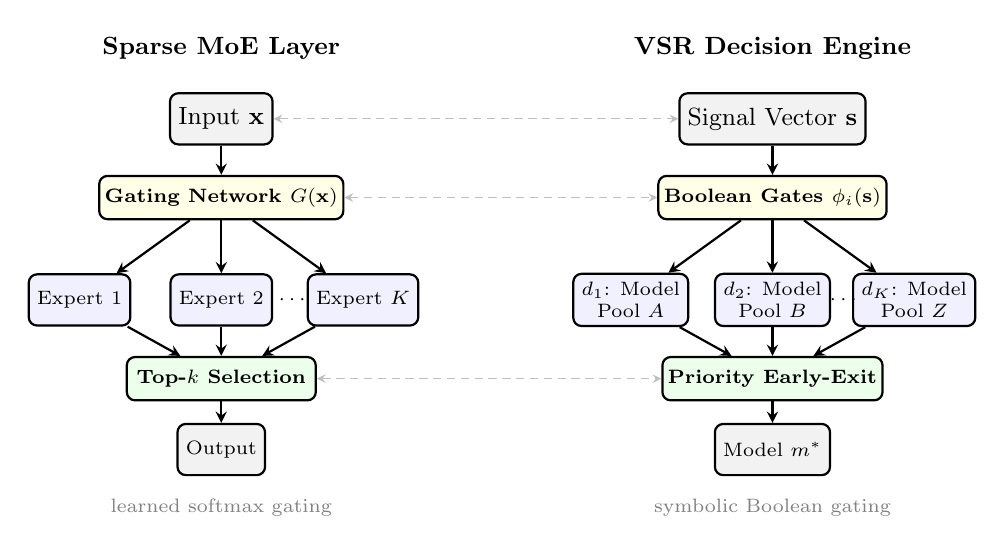
\begin{tikzpicture}[
    box/.style={rectangle, draw, thick, rounded corners=3pt,
                minimum height=0.65cm, align=center, inner sep=3pt, font=\small},
    gate/.style={rectangle, draw, thick, rounded corners=3pt,
                 minimum height=0.55cm, align=center, inner sep=2pt, font=\scriptsize\bfseries},
    arr/.style={->, >=stealth, thick},
    darr/.style={<->, >=stealth, densely dashed, gray!50, thin},
    lbl/.style={font=\scriptsize, text=gray},
  ]

  % === MoE (left) ===
  \node[font=\small\bfseries] at (3.0, 4.0) {Sparse MoE Layer};

  \node[box, fill=black!5] (mx) at (3.0, 3.1) {Input $\mathbf{x}$};
  \node[gate, fill=yellow!10, minimum width=2.4cm] (mg) at (3.0, 2.1) {Gating Network $G(\mathbf{x})$};

  \node[box, fill=blue!6, font=\scriptsize] (me1) at (1.2, 0.8) {Expert 1};
  \node[box, fill=blue!6, font=\scriptsize] (me2) at (3.0, 0.8) {Expert 2};
  \node[box, fill=blue!6, font=\scriptsize] (me3) at (4.8, 0.8) {Expert $K$};
  \node[font=\scriptsize] at (3.9, 0.8) {$\cdots$};

  \node[gate, fill=green!8, minimum width=2.4cm] (msel) at (3.0, -0.2) {Top-$k$ Selection};
  \node[box, fill=black!5, font=\scriptsize] (mout) at (3.0, -1.1) {Output};

  \draw[arr] (mx) -- (mg);
  \draw[arr] (mg) -- (me1);
  \draw[arr] (mg) -- (me2);
  \draw[arr] (mg) -- (me3);
  \draw[arr] (me1) -- (msel);
  \draw[arr] (me2) -- (msel);
  \draw[arr] (me3) -- (msel);
  \draw[arr] (msel) -- (mout);

  \node[lbl, anchor=north] at (3.0, -1.6) {learned softmax gating};

  % === VSR Decision Engine (right) ===
  \node[font=\small\bfseries] at (10.0, 4.0) {VSR Decision Engine};

  \node[box, fill=black!5] (vs) at (10.0, 3.1) {Signal Vector $\mathbf{s}$};
  \node[gate, fill=yellow!10, minimum width=2.4cm] (vg) at (10.0, 2.1) {Boolean Gates $\phi_i(\mathbf{s})$};

  \node[box, fill=blue!6, font=\scriptsize] (vd1) at (8.2, 0.8) {$d_1$: Model\\Pool $A$};
  \node[box, fill=blue!6, font=\scriptsize] (vd2) at (10.0, 0.8) {$d_2$: Model\\Pool $B$};
  \node[box, fill=blue!6, font=\scriptsize] (vd3) at (11.8, 0.8) {$d_K$: Model\\Pool $Z$};
  \node[font=\scriptsize] at (10.9, 0.8) {$\cdots$};

  \node[gate, fill=green!8, minimum width=2.4cm] (vsel) at (10.0, -0.2) {Priority Early-Exit};
  \node[box, fill=black!5, font=\scriptsize] (vout) at (10.0, -1.1) {Model $m^*$};

  \draw[arr] (vs) -- (vg);
  \draw[arr] (vg) -- (vd1);
  \draw[arr] (vg) -- (vd2);
  \draw[arr] (vg) -- (vd3);
  \draw[arr] (vd1) -- (vsel);
  \draw[arr] (vd2) -- (vsel);
  \draw[arr] (vd3) -- (vsel);
  \draw[arr] (vsel) -- (vout);

  \node[lbl, anchor=north] at (10.0, -1.6) {symbolic Boolean gating};

  % Correspondence arrows
  \draw[darr] (mx.east) -- (vs.west);
  \draw[darr] (mg.east) -- (vg.west);
  \draw[darr] (msel.east) -- (vsel.west);

  \end{tikzpicture}
  \caption{Structural analogy between Mixture-of-Experts gating and the VSR decision engine. \textbf{Left}: In a sparse MoE layer, a learned gating network selects top-$k$ experts via softmax. \textbf{Right}: In VSR, Boolean formulas over the signal vector act as symbolic expert gates, with priority ordering implementing deterministic early-exit selection. Dashed arrows mark the structural correspondence.}
  \label{fig:moe_analogy}
\end{figure}

\subsection{Layered Entropy-Folding Interpretation}
\label{sec:disc_entropy_folding}

The priority-ordered gate stack also admits an information-theoretic interpretation as a layered uncertainty-collapse process.
Let $g_\ell(\mathbf{s}) \in \{0,1\}$ denote the match outcome of the $\ell$-th gate under priority order, and let $Z_\ell = g_\ell(\mathbf{s})$.
Define routing uncertainty after $\ell$ evaluated gates as:
\begin{equation}
  U_\ell = H(M \mid \mathbf{s}, Z_{1:\ell})
\end{equation}
where $M$ is the final selected model random variable.
By the chain rule of mutual information:
\begin{equation}
  U_{\ell+1}
  = U_\ell - I\!\left(M;\, Z_{\ell+1}\mid \mathbf{s}, Z_{1:\ell}\right)
  \le U_\ell
\end{equation}
so each additional gate can only maintain or reduce uncertainty.
In this sense, priority depth is \emph{control depth}: a sequence of policy constraints that folds entropy toward a deterministic choice.

\begin{figure}[!ht]
  \centering
  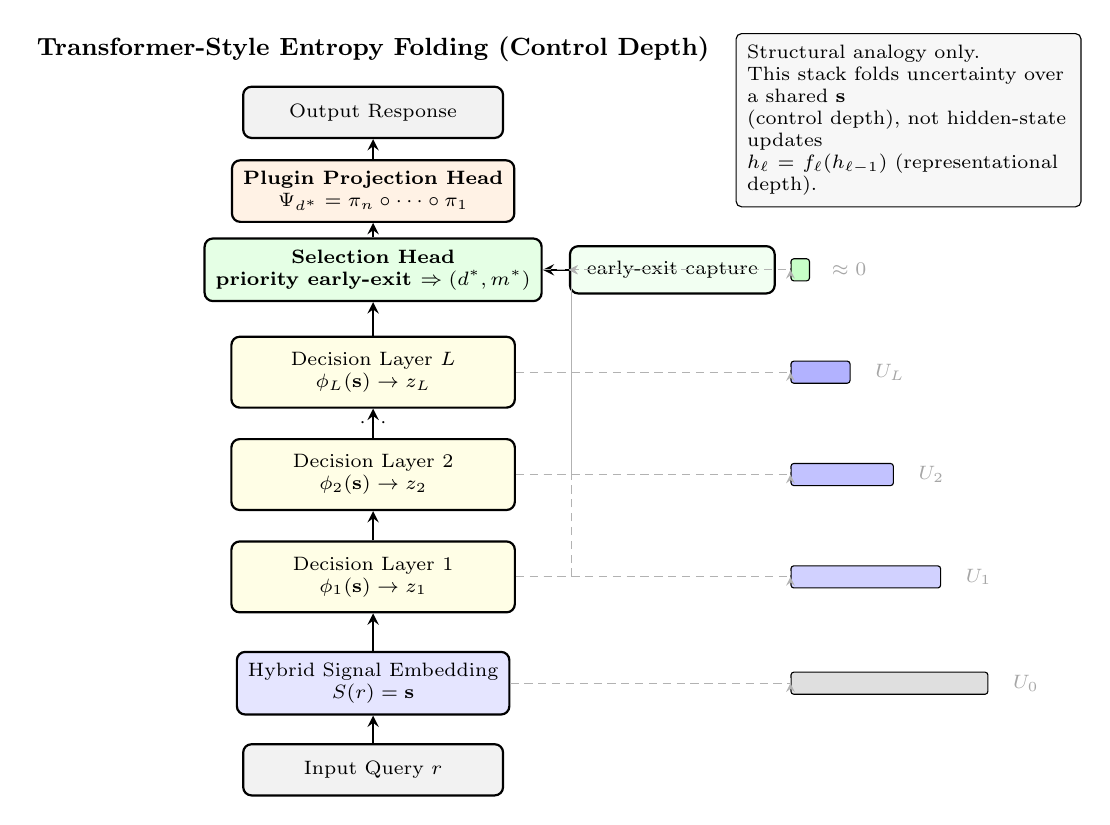
\begin{tikzpicture}[
    box/.style={rectangle, draw, thick, rounded corners=3pt,
                minimum height=0.65cm, minimum width=3.3cm,
                align=center, inner sep=4pt, font=\scriptsize},
    dlayer/.style={rectangle, draw, thick, rounded corners=3pt, fill=yellow!10,
                   minimum height=0.9cm, minimum width=3.6cm,
                   align=center, inner sep=4pt, font=\scriptsize},
    head/.style={rectangle, draw, thick, rounded corners=3pt, fill=green!10,
                 minimum height=0.7cm, minimum width=3.4cm,
                 align=center, inner sep=4pt, font=\scriptsize\bfseries},
    proj/.style={rectangle, draw, thick, rounded corners=3pt, fill=orange!10,
                 minimum height=0.7cm, minimum width=3.4cm,
                 align=center, inner sep=4pt, font=\scriptsize\bfseries},
    arr/.style={->, >=stealth, thick},
    darr/.style={->, >=stealth, densely dashed, gray!60},
    bar/.style={rectangle, draw, rounded corners=1pt, fill=#1, minimum height=0.28cm, anchor=west},
    lbl/.style={font=\scriptsize, text=gray!70},
    note/.style={rectangle, draw, rounded corners=2pt, fill=black!3,
                 text width=4.1cm, align=left, font=\scriptsize, inner sep=4pt}
  ]

  % Title
  \node[font=\small\bfseries] at (3.1, 9.75) {Transformer-Style Entropy Folding (Control Depth)};

  % Main vertical stack
  \node[box, fill=black!5] (inp) at (3.1, 0.6) {Input Query $r$};
  \node[box, fill=blue!10] (emb) at (3.1, 1.7) {Hybrid Signal Embedding\\$S(r)=\mathbf{s}$};

  \node[dlayer] (d1) at (3.1, 3.05) {Decision Layer 1\\$\phi_1(\mathbf{s}) \rightarrow z_1$};
  \node[dlayer] (d2) at (3.1, 4.35) {Decision Layer 2\\$\phi_2(\mathbf{s}) \rightarrow z_2$};
  \node[dlayer] (dL) at (3.1, 5.65) {Decision Layer $L$\\$\phi_L(\mathbf{s}) \rightarrow z_L$};
  \node[font=\scriptsize] at (3.1, 5.0) {$\cdots$};

  \node[head] (sel) at (3.1, 6.95) {Selection Head\\priority early-exit $\Rightarrow (d^*, m^*)$};
  \node[proj] (ph) at (3.1, 7.95) {Plugin Projection Head\\$\Psi_{d^*} = \pi_n \circ \cdots \circ \pi_1$};
  \node[box, fill=black!5] (out) at (3.1, 8.95) {Output Response};

  \draw[arr] (inp) -- (emb);
  \draw[arr] (emb) -- (d1);
  \draw[arr] (d1) -- (d2);
  \draw[arr] (d2) -- (dL);
  \draw[arr] (dL) -- (sel);
  \draw[arr] (sel) -- (ph);
  \draw[arr] (ph) -- (out);

  % Early-exit side path
  \node[box, fill=green!5, minimum width=2.6cm, minimum height=0.6cm] (exit) at (6.9, 6.95) {early-exit capture};
  \draw[darr] (d1.east) -- ++(0.7,0) |- (exit.west);
  \draw[darr] (d2.east) -- ++(0.7,0) |- (exit.west);
  \draw[darr] (dL.east) -- ++(0.7,0) |- (exit.west);
  \draw[arr] (exit.west) -- (sel.east);

  % Entropy folding track
  \node[lbl, font=\scriptsize\bfseries] at (9.6, 7.95) {Entropy Folding};
  \node[bar=gray!25, minimum width=2.5cm] (u0) at (8.4, 1.7) {};
  \node[bar=blue!18, minimum width=1.9cm] (u1) at (8.4, 3.05) {};
  \node[bar=blue!24, minimum width=1.3cm] (u2) at (8.4, 4.35) {};
  \node[bar=blue!30, minimum width=0.75cm] (u3) at (8.4, 5.65) {};
  \node[bar=green!22, minimum width=0.18cm] (uf) at (8.4, 6.95) {};
  \node[lbl, anchor=west] at (11.1, 1.7) {$U_0$};
  \node[lbl, anchor=west] at (10.5, 3.05) {$U_1$};
  \node[lbl, anchor=west] at (9.9, 4.35) {$U_2$};
  \node[lbl, anchor=west] at (9.35, 5.65) {$U_L$};
  \node[lbl, anchor=west] at (8.8, 6.95) {$\approx 0$};
  \draw[darr] (emb.east) -- ++(0.55,0) -| (u0.west);
  \draw[darr] (d1.east) -- ++(0.55,0) -| (u1.west);
  \draw[darr] (d2.east) -- ++(0.55,0) -| (u2.west);
  \draw[darr] (dL.east) -- ++(0.55,0) -| (u3.west);
  \draw[darr] (sel.east) -- ++(0.55,0) -| (uf.west);

  % Boundary note
  \node[note] at (9.9, 8.85)
    {Structural analogy only.\\
     This stack folds uncertainty over a shared $\mathbf{s}$\\
     (control depth), not hidden-state updates\\
     $h_\ell = f_\ell(h_{\ell-1})$ (representational depth).};

  \end{tikzpicture}
  \caption{Transformer-style visualization of layered control depth in VSR.
  Signal extraction constructs a shared embedding $\mathbf{s}$; stacked decision layers apply Boolean gates $\phi_\ell(\mathbf{s})$ that progressively reduce routing uncertainty $U_\ell$; selection resolves $(d^*,m^*)$ via priority early-exit; plugin composition $\Psi_{d^*}$ acts as an output-side projection head over request/response behavior.}
  \label{fig:entropy_folding_layers}
\end{figure}

The MoE analogy also clarifies what the system is \emph{not}: it is not a Transformer in the sequential sense.
Transformer blocks transform the representation layer by layer---each block's output is the next block's input.
In our architecture, all decision blocks operate on the \emph{same} shared signal vector~$\mathbf{s}$; there is no inter-decision information flow.
The priority ordering is an \emph{early-exit mechanism} over parallel evaluations, not a sequential transformation pipeline.
This distinction is important: it means that adding or removing decisions does not affect the behavior of other decisions (modulo priority reordering), a composability property that sequential architectures lack.
